\documentclass[letterpaper,10pt,conference]{ieeeconf}
\overrideIEEEmargins
\usepackage[T1]{fontenc}
\usepackage[utf8]{inputenc}
\usepackage{amsmath,amssymb,graphicx,booktabs,cite,xcolor}
% Official class and margins are unmodified. No author identifiers or active URLs.
\pdfinfo{/Author () /Subject (Anonymous working draft) /Keywords (procedural environments, robot navigation)}
\newcommand{\todo}[1]{\textcolor{red!65!black}{\textbf{TODO:} #1}}
\newcommand{\missing}{\textemdash}
\newcommand{\resultplaceholder}[2]{\textcolor{red!65!black}{[\textbf{#1}: #2]}}
\title{\LARGE\bf CAVERN: Controllable and Validated Environments for Robotic Navigation in Underwater Caves}
\author{Anonymous Authors}
\begin{document}
\maketitle
\thispagestyle{empty}\pagestyle{empty}
\begin{abstract}
Training and evaluating cave-navigation policies require environment variation whose effects can
be distinguished from changes in task feasibility. A connected cave skeleton
alone does not establish that a finite-sized robot can reach a goal through the
generated surfaces. We introduce Cave Composer, a task-conditioned procedural
generator for cave navigation, with underwater visual navigation as its target
application. The generator combines explicit structural controls with irregular
cross-sections and localized geometric changes around a protected passage.
This passage reserves space for a spherical robot envelope, a safety margin
and a discretization allowance. Within each cave, multiple start--goal requests
are searched on a three-dimensional occupancy grid without using the construction
centerline as a planner input. Candidate paths undergo inside and
spacing-corrected clearance checks on both extracted visual and collision meshes.
Scene and task seeds make the resulting environments and requests reproducible.
\resultplaceholder{RESULT-GEOM}{State the tested geometric claim, comparison,
independent sample unit, measured result and uncertainty.}
\resultplaceholder{RESULT-NAV}{Report the measured effect of environment design
within each baseline on specified held-out tasks, including uncertainty; do not
assume improvement.}

\end{abstract}
\section{Introduction}
\begin{figure*}[t]
\centering
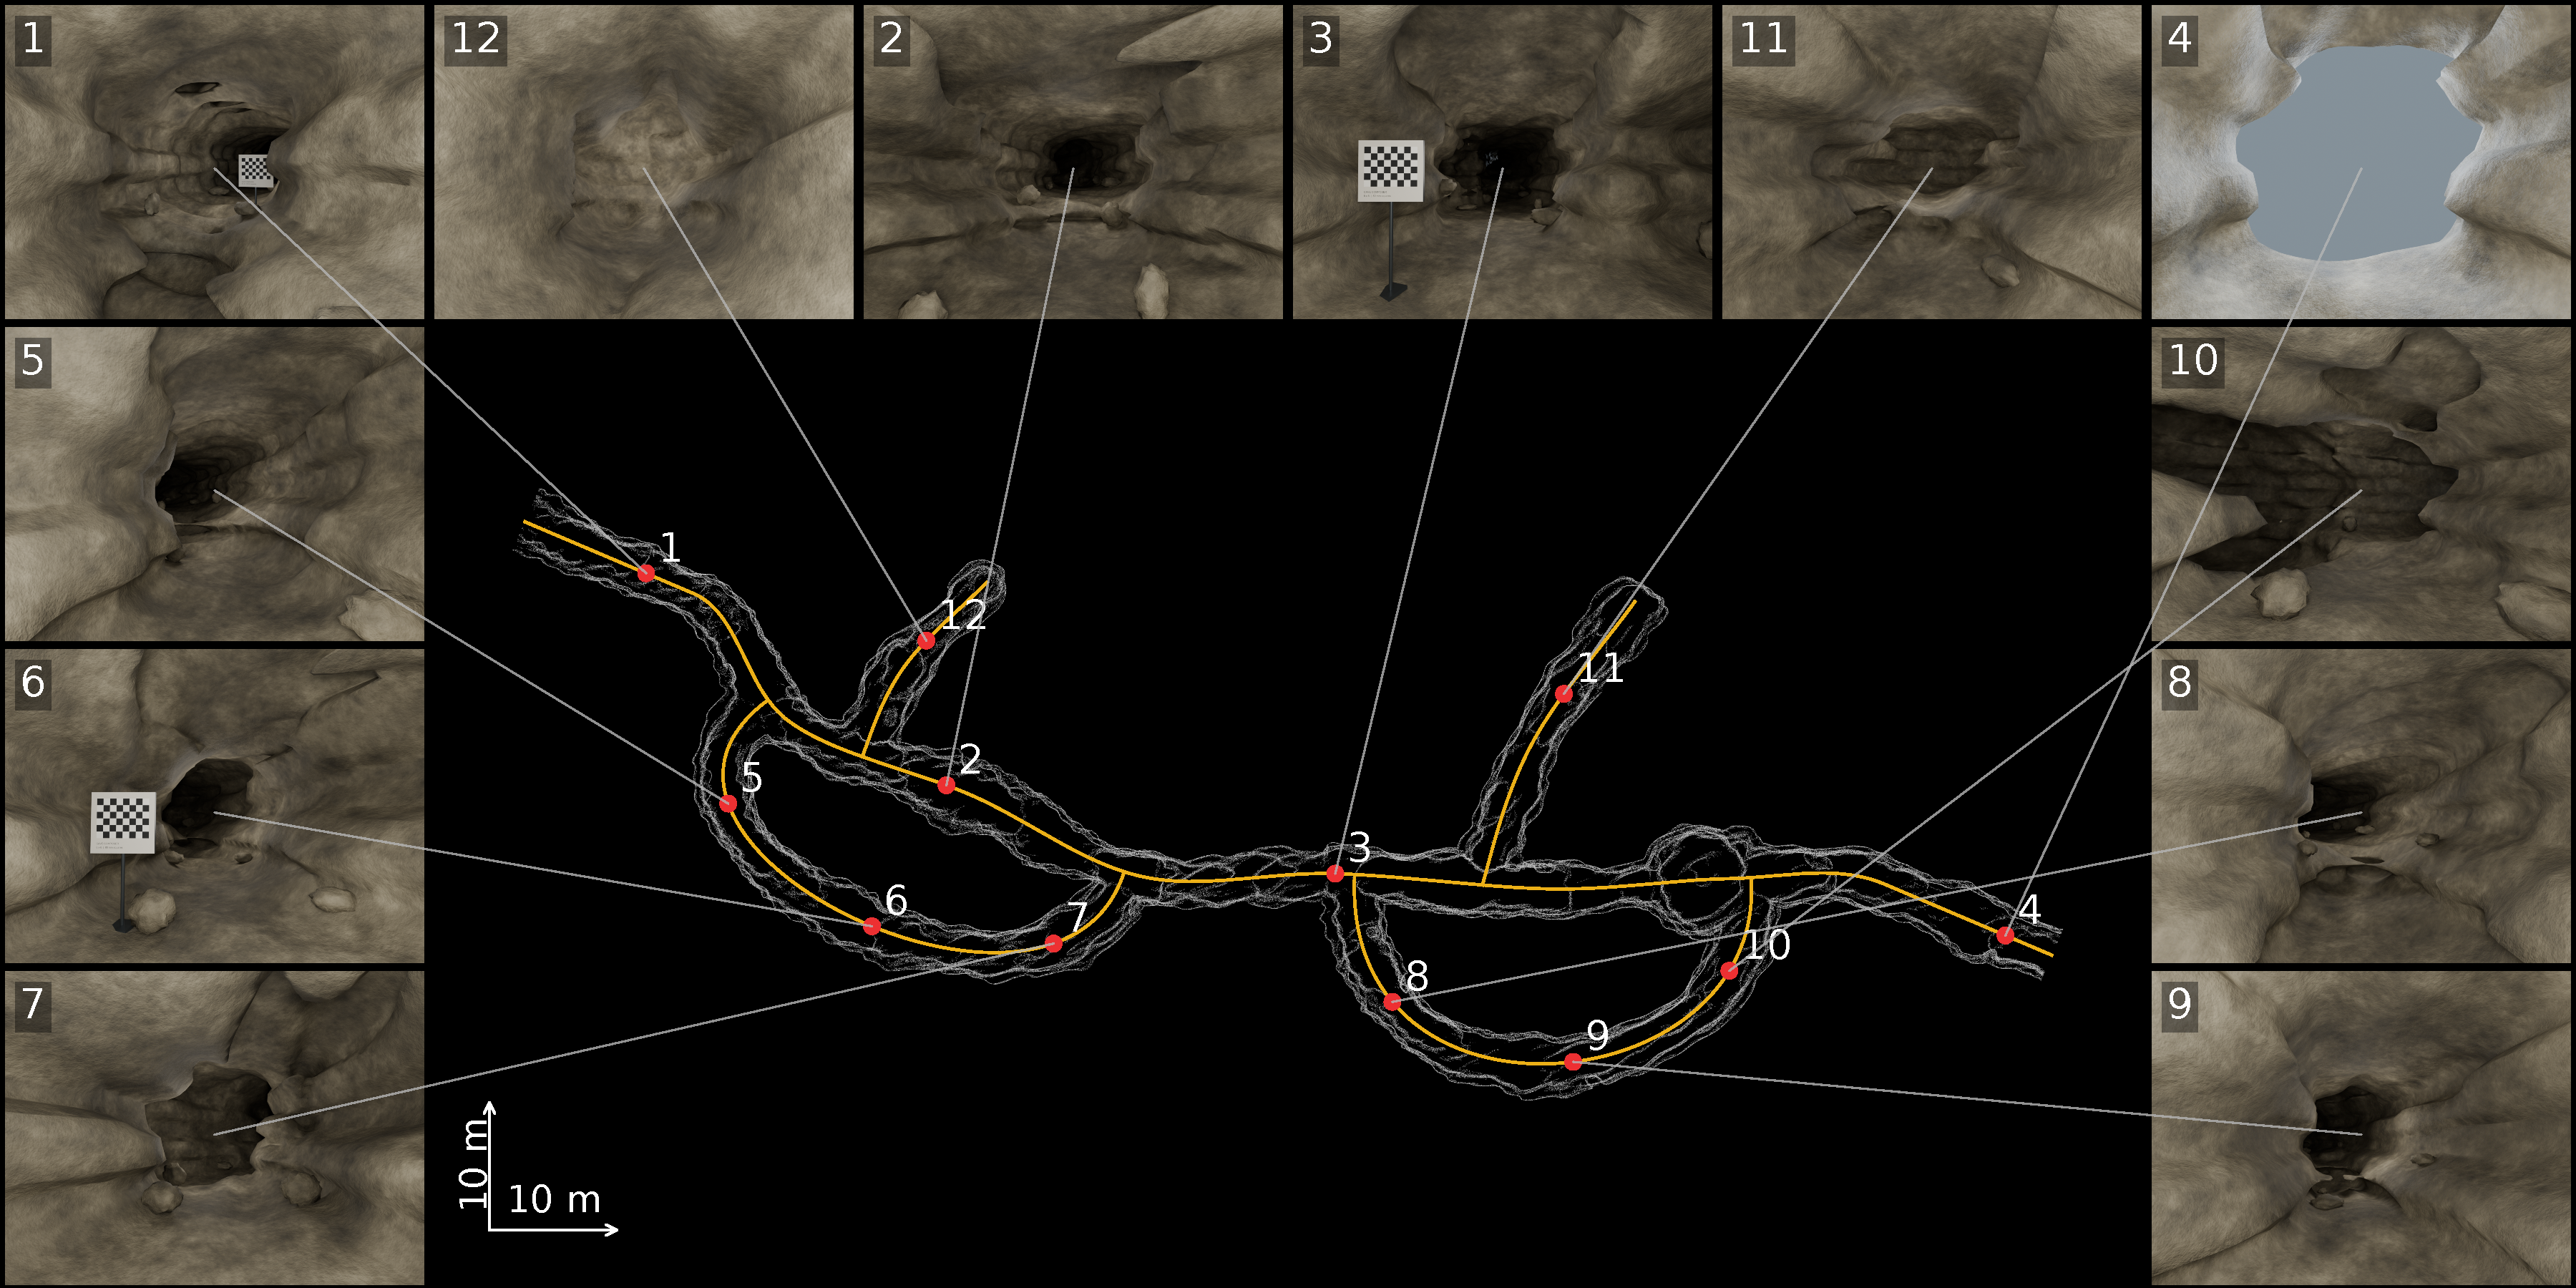
\includegraphics[width=\textwidth]{figures/showcase_hard_v02/cave_showcase.pdf}
\caption{A complex cave generated by Cave Composer, with two rejoining loops
and two blind branches. Twelve Blender interior views are linked to their
camera locations (red) on a mesh-sampled overview; yellow lines show
construction centerlines. Rocks and checkerboard props add local visual detail.
The views use inspection lighting without a water medium. The overview and
centerlines depict generated structure, not a sensor reconstruction or an
executed robot trajectory.}
\label{fig:cave-showcase}
\end{figure*}

The environments used to train a cave-navigation policy determine which
junctions, constrictions and obstacles it encounters, and which failures its
evaluation can reveal. For underwater visual navigation, this makes cave
geometry a central experimental variable alongside sensing and vehicle dynamics.
Changing a passage's shape can simultaneously alter its visual appearance,
occlusion and clearance. If an environment variation blocks the specified robot,
a failed episode no longer isolates the navigation policy's ability to handle
that variation. Conversely, a set of wide, repetitive passages offers limited
coverage of the geometric situations of interest. We study controllable cave
environment generation, with underwater navigation as the motivating application.
Figure~\ref{fig:cave-showcase} illustrates the passage structure and local
appearance of one generated cave.

Procedural generation already supports both environmental diversity and
constraints on usable space. ProcTHOR generates houses and checks agent
reachability after construction~\cite{deitke2022procthor}; Infinigen Indoors
and Holodeck impose constraints on scene composition~\cite{raistrick2024indoors,yang2024holodeck}.
For caves and tunnels, implicit modeling, geological controls and graph-based
authoring provide branching layouts and varied passage
geometry~\cite{raistrick2023infinigen,paris2021caves,cano2024tunnels,garcia2025plume}.
The problem addressed here lies at the intersection of these capabilities:
linking controlled changes in cave structure and local morphology to a specified
robot envelope and start--goal task on the resulting geometry. A desired layout,
a nominal passage width and a path through the final cave describe different
properties; navigation experiments need an explicit relationship between them.

Our central design separates preserving space during generation from establishing
a task's geometric feasibility afterward. A protected passage limits how far
local geometric changes can intrude into the intended route. Surface extraction
and the choice of collision resolution still affect the resulting boundary,
and different endpoint pairs need their own paths. Thus, generation-time
protection supplies a useful construction constraint, while post-generation
checks determine which tasks satisfy the requested clearance on the meshes
actually produced. This separation permits irregular geometry without treating
the generator's own skeleton as evidence of task feasibility.

We introduce \emph{Cave Composer}, a task-conditioned procedural generator for
cave navigation (Fig.~\ref{fig:method}). Structural controls specify turns,
slopes, branches, rejoining passages and chambers; local controls vary sections,
wall intrusions and spatial roughness in an implicit void field. A task sampler
selects multiple start--goal pairs within the same cave. Although construction
routes can guide endpoint selection, the subsequent 3D A* search receives
occupancy and endpoints, not those routes or their graph. Each candidate polyline
is checked for containment and clearance against both extracted visual and
collision meshes, with an allowance for the distance between checked samples.
These checks concern a static spherical envelope on the checked geometry;
dynamic execution and navigation from visual observations are separate questions.

In a paired pilot over six fixed requests, full generation accepts five,
disabling protection accepts four, and restricted generation accepts all six
(Table~\ref{tab:generator}). Protection changes acceptance in one stress case;
another is rejected by both full and unprotected generation. These outcomes
show why acceptance and realized geometric variation must be reported together.
\resultplaceholder{RESULT-GEOM}{State the tested geometric claim,
comparison, independent sample unit, measured result and uncertainty for the
broader generation study.}

Downstream utility concerns the effect of training environments within a fixed
learner and observation setting. A controlled evaluation can use
FlashSAC~\cite{kim2026flashsac} and recurrent visual
PPO~\cite{schulman2017ppo} as separate baselines in an external navigation
platform.
Our contributions are:
\begin{enumerate}
\item We introduce Cave Composer, a controllable cave generator that couples
structural and local geometric variation to robot-dependent passage protection.
Per-task occupancy search and checks on both extracted visual and collision
meshes connect the generated geometry to reproducible navigation tasks.
\item \resultplaceholder{RESULT-NAV}{State the measured effect of training-cave
diversity on held-out navigation performance within each fixed baseline, with
matched observations and training budgets, task definitions and uncertainty.}
\item \resultplaceholder{RESULT-TRANSFER}{State the frozen-policy outcomes on
eligible, previously unseen real-source cave assets in simulation, identifying
task scope, source separation, uncertainty and limitations.}
\end{enumerate}

\section{Related Work}
\subsection{Procedural and controllable 3D environments}
Procedural scene generators reduce the manual effort of assembling varied
training worlds, but they differ in what their controls describe. ProcTHOR
combines room layouts, assets and object placement to produce interactive houses
for embodied learning~\cite{deitke2022procthor}. Its post-generation validator
uses reachable agent positions to check access to every room. This provides a
precedent for coupling procedural generation with agent-specific reachability.
Our geometric question concerns a different setting: three-dimensional paths for a specified
spherical envelope through irregular cave boundaries represented by separate
visual and collision meshes.

Control also extends beyond selecting a random seed. Infinigen generates
natural scenes through procedural geometry and materials, exposing parameters
that determine scene content~\cite{raistrick2023infinigen}. Infinigen Indoors
adds a language for composition constraints, a solver for arranging procedural
assets, and export to real-time simulators~\cite{raistrick2024indoors}.
Holodeck translates language descriptions into scene designs and spatial
relations between retrieved objects, then optimizes their
placement~\cite{yang2024holodeck}. These approaches establish ways to connect
user intent to geometry, spatial constraints and embodied environments.
Cave Composer concentrates its controls on the cavity itself: passage structure,
local wall shape and clearance relative to a robot. Scene composition and
robot-clearance conditions are complementary forms of control.

\subsection{Underground and cave environment generation}
Cave modeling has long addressed geometry beyond smooth, uniform tunnels.
Paris et al. construct karst networks from geological conditions and
inlet--outlet information, then model conduits with implicit primitives,
blending and warping~\cite{paris2021caves}. Their method controls both network
structure and cross-section geometry. Infinigen's cave generator likewise uses
probabilistic production rules for turns, elevation changes and forks, and
combines passages with varying cross-sections through implicit
geometry~\cite{raistrick2023infinigen}. Geological coherence and geometric
variety are therefore substantive prior capabilities. Our emphasis is on
conditioning these kinds of variation on a robot's required clearance and
checking the resulting start--goal tasks; geometric resemblance to real caves
is a separate property to measure.

Robotics-oriented underground generators connect structural representations
to reusable simulation geometry. Cano et al. generate tunnel meshes from a
graph and support automated workflows across multiple simulated
environments~\cite{cano2024tunnels}. PLUME separates graph construction,
meshing and texturing, supports single- and multi-layer underground layouts,
and accepts user-supplied graphs~\cite{garcia2025plume}. Its procedural
materials, texture baking and scene export support robotic simulation across
varied passages and chambers. These systems supply important precedents for
automating underground environment creation. Cave Composer organizes its
pipeline around the relationship between that generated environment and each
sampled task: an explicit protected passage constrains generation, an occupancy
search proposes a path without consuming the construction graph, and both
mesh representations participate in acceptance. The comparison concerns how
requested morphology and clearance relate to accepted tasks on the resulting
geometry.

\subsection{Environment design and generalization}
Environment variation matters because a learner can fit its training worlds
without succeeding on held-out tasks. Procgen studies this issue with procedural
environment distributions and separate assessments of sample efficiency and
generalization~\cite{cobbe2020procgen}. Domain randomization varies rendering
conditions to support visual transfer from simulation~\cite{tobin2017randomization}.
For cave navigation, these perspectives motivate distinguishing appearance
variation from structural and geometric variation. Cave Composer assigns
appearance a separate seed, allowing texture selection to vary while a cave's
geometry and task remain fixed. Such controls define interventions for studying
environment design; a new seed alone does not define an out-of-distribution test.

Unsupervised environment design goes further by adapting the training
distribution to the learner. PAIRED uses a protagonist, an antagonist and an
environment adversary, with a regret-based objective that favors challenging,
solvable environments~\cite{dennis2020paired}. Structured, solvable task
distributions are thus an established research objective. Cave Composer instead
specifies cave geometry and task acceptance through explicit conditions and
geometric checks, independently of policy returns. It provides an environment
family within which the effects of chosen training conditions can be studied.
This places the learning question on the environment distribution: comparisons
should vary that distribution within each fixed baseline, rather than attribute
differences between learning algorithms to the generator.

\subsection{Underwater simulation}
Underwater simulators model the sensing and dynamics through which cave geometry
becomes a robot's experience. Stonefish supplies marine-robot physics, sensors
and rendering~\cite{cieslak2019stonefish}; OceanSim emphasizes GPU-accelerated,
physics-based underwater visual and acoustic sensor
simulation~\cite{song2025oceansim}. Isaac Lab provides a broader framework for
parallel robot learning~\cite{nvidia2025isaaclab}. These platforms are
complementary to Cave Composer's environment-generation role. Their vehicle and
sensor models provide the physical and perceptual conditions under which a
generated cave can be evaluated. Cave Composer supplies controlled geometry and
geometrically checked tasks for such evaluations. Studying environment design
with existing learners therefore requires a specified vehicle and observation
model in addition to geometric feasibility.

\section{Cave Composer}
\begin{figure*}[t]
\centering
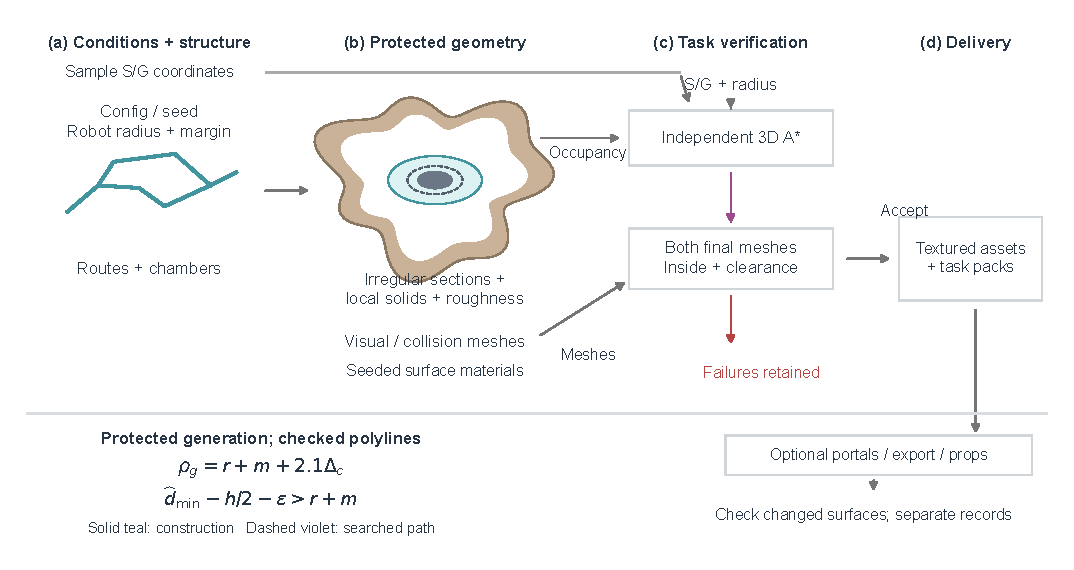
\includegraphics[width=\textwidth]{figures/generated/cave_composer_method.pdf}
\caption{Cave Composer pipeline. Construction routes condition geometry
and endpoint sampling; only occupancy, endpoints and the required radius feed
the independent search. Candidate paths are checked on both final meshes.
Portal/export and post-generation obstacle checks are distinct from the
closed-reference certificate. The lower detail illustrates protection and
the spacing-corrected distance bound. Lines denote construction or geometric
witnesses, not executed robot trajectories.}
\label{fig:method}
\end{figure*}
\subsection{Conditions and intended structure}
A scene request contains structural conditions $c$, a scene seed $s$, and
a spherical robot radius $r$ with margin $m$. The route grammar represents
straight segments, controlled turns and elevation changes, with branches,
rejoining passages and chambers. Later optional sampling presets introduce
curved meanders, dead ends and asymmetric loops. Nominal widths and heights
are controls, not measurements of every local opening. Bounded layout screening
rejects unsuitable route proximity and voxel-budget requests before meshing;
it does not certify the topology of the final free space.

\subsection{Irregular geometry with passage protection}
The generator composes an implicit void field from route-dependent sections
and chambers. Optional morphology controls introduce eccentric section
variation, side cavities, ceiling drops, floor rises, wall intrusions,
overhangs and rockfall-like obstacles. A spatial modulation field changes
roughness across the cave. These mechanisms have separate parameters;
adding uniform high-frequency noise cannot substitute for section asymmetry
or localized solid obstacles.

Let $d_C(x)$ denote the distance approximation to the construction route used
by the generator and $F_{\mathrm{var}}(x)$ its varied void field. Positive field
values denote void. Both terms below are distance-like scalars expressed in
metres, although neither the varied field nor their maximum is an exact SDF.
The maximum is an implementation rule for union of positive regions; acceptance
of the discretized output is determined by final-mesh checks. The rule is
\begin{equation}
\begin{aligned}
F(x)&=\max\{F_{\mathrm{var}}(x),\rho_g-d_C(x)\},\\
\rho_g&=r+m+2.1\Delta_c,
\end{aligned}
\end{equation}
where $\Delta_c$ is the collision-grid spacing. The additional allowance is an
implementation choice for discretization, not a sharp universal error bound.
Final geometric checks remain necessary. The field is not an exact signed
distance function. Surface extraction at separately specified resolutions
produces visual and collision meshes. Their common intended layout does not
make their clearances identical.

\subsection{Independent task search and final-mesh checks}
A task seed selects a fixed budget of start--goal requests within one cave.
The semantic routes may select endpoints, including branch interiors.
The search itself consumes occupancy, grid coordinates, endpoints and the
required radius $\rho=r+m$. It uses a conservative distance transform and
six-neighbor, clearance-weighted A*. No centerline or semantic graph is an
input to this search. Failure under its discretization or search budget does
not prove that all possible continuous paths are infeasible.

For each candidate polyline $P$, samples include its vertices and have maximum
adjacent spacing $h$. On each final mesh $M$, let $d_{\min}(M)$ be the smallest
sampled point-to-triangle distance. Since distance to a fixed surface is
1-Lipschitz, every point of a sampled segment lies within $h/2$ of a sample,
giving the lower bound
\begin{equation}
\inf_{x\in P}d(x,M)\ \geq\ d_{\min}(M)-h/2\ >\ r+m.
\label{eq:clearance}
\end{equation}
Here the analytic bound uses exact distances. The implementation subtracts
an additional tolerance $\epsilon\geq10^{-6}$\,m from computed distances before
testing $\widehat d_{\min}-h/2-\epsilon>r+m$. This is an explicit engineering
allowance, not an interval-arithmetic rounding-error proof. Non-watertight or
inconsistently wound references are rejected before parity is evaluated.
Inside tests assume a valid closed cavity boundary; separate intersection
audits are still needed. Acceptance
requires both visual and collision checks. The bound applies to a spherical
static envelope and does not certify dynamics, tracking error or perception.
Each request retains its outcome; failed tasks are not replaced to inflate
the accepted fraction.

\subsection{Exports, appearance and modified surfaces}
Materials use a separate appearance seed. Optional reviewed scan-color patches
have source-group records; they do not establish a fitted geometric prior or
recover physical reflectance. Portable texture exports retain the association
between geometry, material and hashes.

Portal cutting is a separate deterministic export from a closed reference.
The procedural portal checker requires two intentional boundary loops and
tests a crossing path against the resulting open surfaces. Portable-format
checks inspect reimported geometry and coordinates. Showcase obstacles have
their own combined-surface checks. These records are scoped to the path they
actually check. The current portal exporter reuses the independently searched
interior path and adds separately checked straight terminal approaches.
An open export uses unsigned triangle distance, never an open-mesh parity
result. Fresh delivery checks reload both OBJs, merge only exactly coincident
UV-seam vertices without changing triangles, and bind certificates to file
and path hashes. A closed certificate must never silently
carry over to a changed collision mesh, added obstruction or simulator import.
Arbitrary simulator conversion currently requires an additional runtime gate.

\subsection{Reproducibility and geometric evaluation}
Scene and task records include seeds, normalized configuration, file hashes,
code-file hashes, dependency identity and retained failures. The package
version label alone is insufficient: multiple later updates still use the
same version string. Dataset manifests must therefore identify the exact
generator sources that produced their assets.

A local integrity audit recovered 36 accepted task records on three historical
caves, with 12 requested tasks per cave. A separate, later morphology snapshot
contains six checked configurations at one shared scene seed. These are
different versioned evidence sets, not a single benchmark or 36 independent
caves. Integrity replay checks persisted records; it is not a new policy
experiment or a fresh distance computation. The new paired pilot below is a
separate evidence set with fresh checks of delivered geometry.

\section{Navigation Learning Setup}
\begin{figure*}[t]
\centering
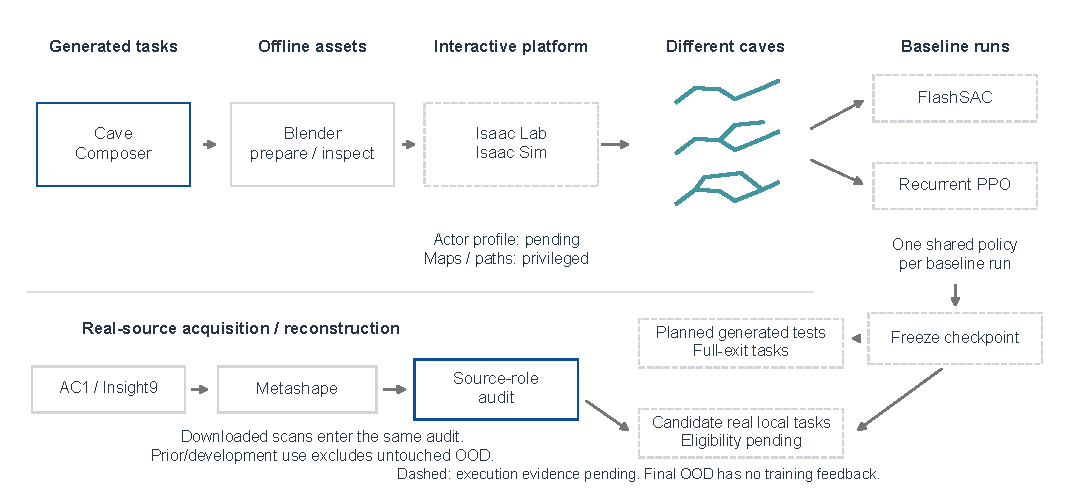
\includegraphics[width=\textwidth]{figures/generated/cavern_framework.pdf}
\caption{Planned experimental architecture. Cave Composer and offline Blender
processing feed distinct cave instances in the external Isaac Lab/Isaac Sim
platform. FlashSAC and recurrent visual PPO are alternative baseline runs;
each run is to use one policy shared across caves. The planned evaluation uses
generated full-exit tasks and candidate real-source local tasks, whose source
eligibility remains unresolved. Real sources
have an audited role before use, and the final-test branch has no feedback
to training. Dashed components require platform evidence; no rendered
miniature represents an Isaac execution screenshot.}
\label{fig:framework}
\end{figure*}
\subsection{Simulation platform and scene integration}
The collaborator reports an underwater visual-navigation platform based on
Isaac Lab. Its configuration, active training manifest and execution logs
are not yet available in this workspace. The local handoff copies verified
task packs to a new snapshot, preserves their scene splits and locks hashes.
A separate smoke test actually ran two different final cave meshes in the
existing Isaac Sim 5.0 installation, with 80\,m-separated instance origins.
Reset positions, static nonconvex triangle collision and namespace-local wall
probes pass. Synchronized 1280$\times$720 RGB pairs use the task-pack 0.12\,m
baseline and intrinsics. An initial dark-image attempt is retained; diagnostic
lamp exposure was corrected before the final check. The test uses direct USD
mesh construction, not Isaac Lab, a vehicle controller or a learned policy.
It does not validate all eight assets in the simulator. Each status distinguishes implementation,
geometry, adapter checks, simulator execution and policy evaluation.

For heterogeneous parallel training, an instance must reference its own cave
asset and task, rather than instantiate the same cave under different IDs.
A proposed sampler selects a cave uniformly and then a task within that cave.
All selected caves share a common policy for a given algorithm, configuration
and training seed. Scene identity is logging metadata, not a selector for
cave-specific policies. Per-instance transforms must move meshes, reset poses,
goals and cameras consistently.

\subsection{Observations and actions}
Historical packs specify stereo RGB sensors but leave goal conditioning and
actions unspecified. Later collaborator descriptions also mention goal or
exit instructions, IMU, pressure, previous actions and localization. The
new profile records these differences instead of modifying historical packs.
All fields of the proposed integration remain \texttt{UNCONFIRMED} until
the actual platform configuration is supplied.

Our provisional profile pairs stereo RGB with a relative goal in the body
frame, inertial and pressure measurements, and the previous action. Computing
the relative goal from simulator ground-truth pose makes this a
\emph{localization-assisted} condition, not RGB-only navigation. Global maps,
construction routes and witness paths remain privileged. The action proposal
is a normalized six-dimensional body-velocity command; actuator conversion,
limits, timing and underwater vehicle dynamics require platform confirmation.
No control or sensor-accuracy result follows from writing this interface.

\subsection{Learning baselines and task configuration}
FlashSAC and recurrent visual PPO are planned as separate baselines, each with
one cross-cave policy. Their visual encoders, memory states, optimizer settings,
normalizers and inference rules must be versioned in each imported run receipt.
The planned experiments change training
environment conditions within one baseline before comparing across baselines.
A handoff records scene and source group, assets, units, pose convention,
robot envelope, resets, goals and task budget. Evaluation receipts identify
the frozen checkpoint, data version and every scheduled episode, including
episodes not executed. Missing data never becomes a zero or an omitted failure.
The actual Isaac Lab and vehicle configuration, remaining asset-instance tests,
and matched training/evaluation receipts are still pending.

\section{Experimental Evaluation}
\subsection{Geometric validity and generation cost}
We executed six fixed base requests under three conditions: full Composer,
the same request with the protected union disabled, and a restricted generator
with oval sections, no branches/chambers and no geometric modifiers. Four
requests are normal cases; two are declared intrusion/roughness stress cases.
All 18 attempts use a 0.35\,m sphere plus 0.20\,m margin, visual/collision
voxel sizes 0.24/0.32\,m, a four-million-voxel ceiling and a 300\,s invocation
budget. There are no replacement seeds or generation retries. Explicit layouts
do not invoke stochastic layout screening, so this is not a screening ablation.

The initial delivery importer retained OBJ texture-seam vertices and rejected
the visual boundary as non-watertight. We declared an importer amendment,
merged only exactly coincident positions and rechecked the same immutable
triangles. Table~\ref{tab:generator} reports these corrected outcomes; the
original rejections remain archived. All three conditions accept 4/4 normal
requests. On the two stress requests, Composer accepts 1/2, no protection 0/2,
and restricted 2/2. One stress request produces a large disconnected void
component under both full and unprotected generation and is rejected. The
other unprotected request has endpoints outside the conservative robot grid.
Thus protection helps one retained stress case, while the restricted geometry
has higher overall yield in this pilot. Six purposively fixed requests are
insufficient for a statistical advantage or robustness claim.
Figures~\ref{fig:pilot} and~\ref{fig:protection} show the aggregate outcomes
and the retained protection diagnostic, respectively.

Seventeen fixed transverse planes per delivered mesh measure enclosing
section span, area, nonconvexity and centroid-direction proxies. These
measurements include junctions and chambers: they expose the difference between
nominal construction dimensions and actual geometry, rather than demonstrate
accurate diameter tracking. Full normal outputs retain the requested branch
and chamber cases and nonuniform sections; the restricted outputs omit these
mechanisms. No exact free-space branch/loop count or real-cave distribution
match is established. Wall-clock costs include failed attempts, both import
checks and measurements on a shared workstation, not isolated throughput.
Figure~\ref{fig:cases} separates geometric appearance from texture changes.

A separate analytic fixture suite detects four injected faults: a thin slab,
a local cap, a visual-only slab and a post-export width contraction below the
robot diameter. Both analytically clear controls pass. Labels follow explicit
box/slab inequalities, not checker outputs. This six-fixture diagnostic is not
an estimate of arbitrary-mesh detector accuracy. Disabling generation protection
changes geometry; bypassing this checker would instead change acceptance.

Actual PLUME native and supported graph-input smoke runs were attempted on
a pinned upstream revision. Native execution was blocked by the Windows
\texttt{noise} build dependency; graph input reached upstream mesh generation
but failed at an incompatible Blender 5.2 geometry-node API. No comparable
PLUME yield or timing is reported, and unsupported settings are not counted
as algorithmic failures.
\begin{table}[t]
\centering
\caption{Descriptive generation pilot, after declared OBJ seam recheck. Costs include failed attempts and both delivery checks. PLUME comparison was blocked.}
\label{tab:generator}
\small
\begin{tabular}{lccc}
\toprule
Condition & Normal & Stress & s / accepted \\
\midrule
Composer & 4/4 & 1/2 & 11.12 \\
No protection & 4/4 & 0/2 & 12.72 \\
Restricted & 4/4 & 2/2 & 4.76 \\
PLUME & \missing & \missing & \missing \\
\bottomrule
\end{tabular}
\end{table}

\begin{figure*}[t]
\centering
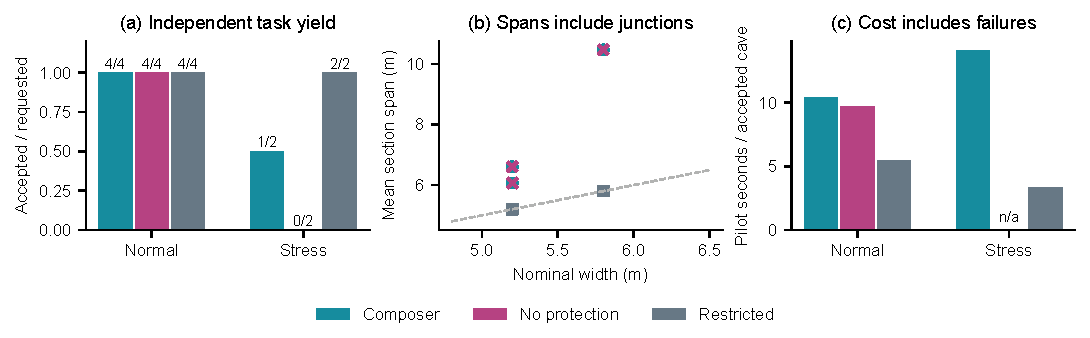
\includegraphics[width=\textwidth]{figures/generated/c1_v02/pilot_quantitative.pdf}
\caption{Descriptive generation pilot after the declared exact-position OBJ seam
recheck: six base requests, eighteen single attempts. Section spans include
junctions and chambers and are not precise diameter-control errors. Cost
includes failed attempts and measurement; no-protection stress cost per
accepted cave is undefined because neither request passed. No policy or PLUME
comparison is represented.}
\label{fig:pilot}
\end{figure*}
\begin{figure*}[t]
\centering
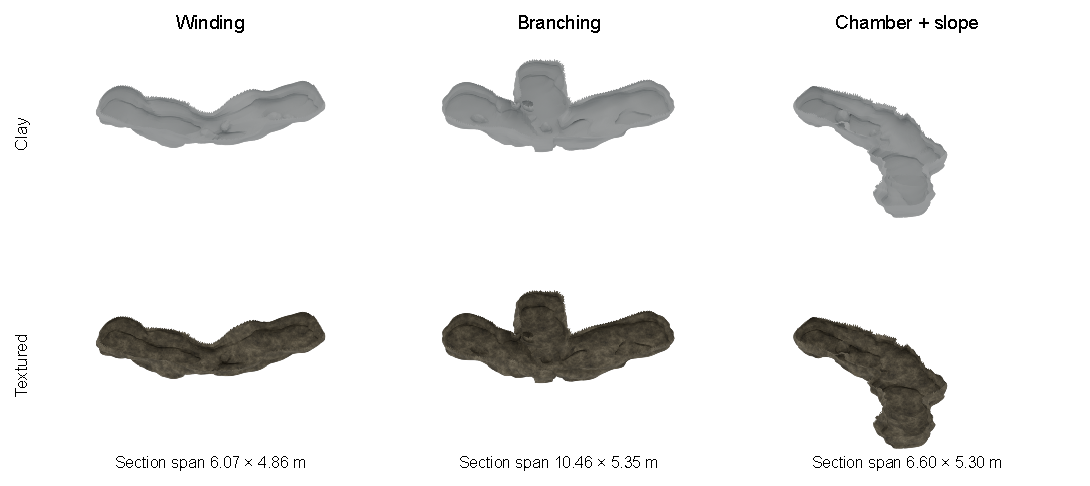
\includegraphics[width=\textwidth]{figures/generated/c1_v02/fixed_cave_cases.pdf}
\caption{Three fixed normal pilot requests, rendered from actual meshes with
the same orthographic scale and view. Clay and textured rows share geometry
and flat normals. Roof removal is an inspection cutaway only. Labels are
mean transverse section spans on delivered visual meshes, including junctions
and chambers; they are not nominal configuration values.}
\label{fig:cases}
\end{figure*}
\begin{figure*}[t]
\centering
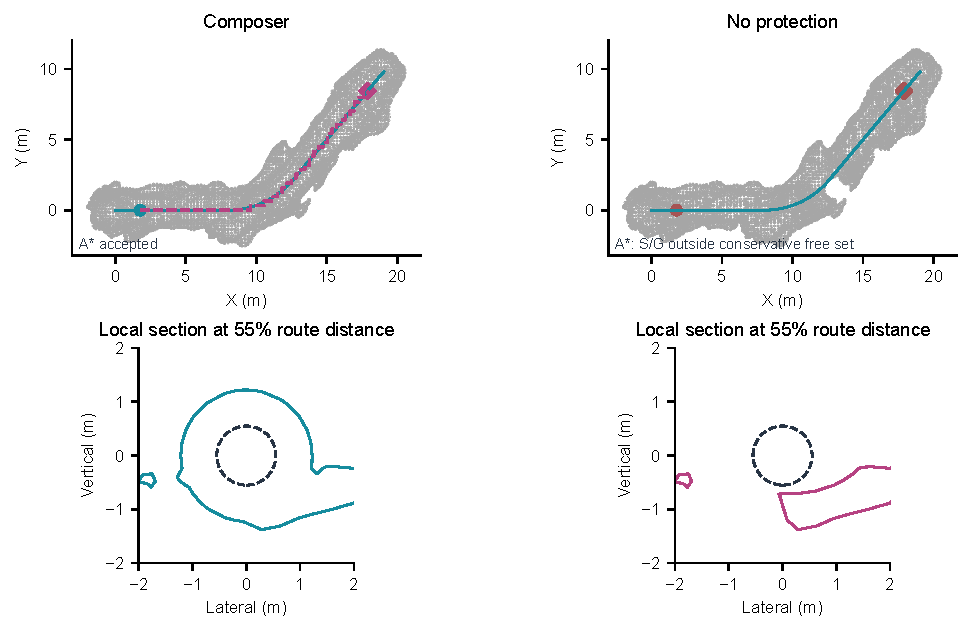
\includegraphics[width=.88\textwidth]{figures/generated/c1_v02/protection_actual_geometry.pdf}
\caption{Fixed stress request with and without passage protection. Gray points
are projections of actual triangle centroids, not a sensed point cloud. Teal
is the construction route; the dashed magenta curve is an independently
searched path, not a robot trajectory. The unprotected mesh is a retained
failed diagnostic: both red endpoint markers fail the conservative-grid gate,
which does not prove continuous-space infeasibility. Matched local sections
at 55\% of the sampled route show geometric change; the dashed circle is the
0.55\,m robot-plus-margin envelope. These sections are distinct from the
endpoint rejection locations.}
\label{fig:protection}
\end{figure*}

\subsection{Effect of training environments}
For each baseline separately, train on restricted caves and full Composer
caves under equal interaction, scene and observation budgets. Fix the
implementation, encoder, memory, vehicle and optimization choices within this
comparison, and report wall time separately from environment interactions.
Use multiple independent training seeds; choose the final count and budget
before launch. A fixed generated validation split selects checkpoints and
hyperparameters. Retention across previously encountered cave families is
evaluated with fixed episodes, without retraining a cave-specific policy.

The new interface pilot contains eight scenes, four per condition: two train,
one development and one generated-ID-test scene per condition. All derivatives
and episodes of a base cave share its split across conditions. Twenty-four
fixed episodes comprise sixteen interior pairs and eight portal full-exit
tasks. The primary paired schedule uses one common interior request and one
exit task per scene; eight auxiliary interior tasks are retained separately.
New seeds define new ID geometry, not automatic OOD.

Nominal geometry, robot size, appearance seed and primary request counts are
matched; realized path clearances still differ between conditions and are
reported per pair. This delivery is therefore an interface pilot, not a fully
clearance-matched causal training comparison. Initial portal export records
retain one boundary-overlap alarm. A uniform 5\,cm terminal-inset revision
passes all eight portable texture/geometry checks. Fresh checks cover internal
paths and ordered entrance/exit witnesses on both changed surfaces. Historical
training snapshots remain separate. No learning curve or policy result is
available (Table~\ref{tab:navigation}).
\begin{table}[t]
\centering
\caption{Planned navigation evaluation matrix. Within each algorithm, hold
training and observation budgets fixed. Dashes mean no policy result exists.}
\label{tab:navigation}
\small
\begin{tabular}{llcc}
\toprule
Baseline & Training caves & Generated & Real-source \\
 & & full exit & local tasks \\
\midrule
FlashSAC & Restricted & \missing & \missing \\
FlashSAC & Composer & \missing & \missing \\
Recurrent PPO & Restricted & \missing & \missing \\
Recurrent PPO & Composer & \missing & \missing \\
\bottomrule
\end{tabular}
\end{table}


\subsection{Frozen-policy transfer on local cave tasks}
Candidate real sources include downloaded scan assets, a team-acquired cave
reconstruction and a reconstruction derived from an external dataset.
The acquisition provenance records AC1/Insight9 and Metashape where reported,
with dates, calibration accuracy and scale left unresolved unless supported
by source records. Local exports are currently uncalibrated open scans.
Underwater simulation on dry-cave geometry is distinct from underwater
acquisition and from executing an embodied robot in the physical cave.

Before policy testing, fix short start--goal segments that cover passage
following, local turns, narrowing or elevation changes. A fragment need not
span the entire cave, but it cannot be selected retrospectively from successful
policy trajectories. Each scheduled episode uses one reset and no manual
correction or dense expert waypoints. The same checkpoint, observation
processing, normalizer and inference rule remain frozen for all assigned
episodes, with no test-time fine-tuning.

All derivatives of one physical cave share a source group, including different
scans, crops, textures and file formats. A source used for materials, geometric
priors, training or generator tuning is ineligible as completely untouched
final OOD. Existing metadata records appearance use for two downloaded cave
groups and development use for the earlier real-data prior. Both newly cropped
reconstructions also have long portions designated for training; actual use
is unconfirmed. Their short portions support within-source spatial holdout,
not an automatic unseen-cave claim. Final source eligibility must be resolved
before transfer can be evaluated.

\subsection{Evaluation metrics and uncertainty}
Record success, collision, out-of-bounds and timeout under a fixed termination
precedence. Keep infrastructure aborts and non-executed episodes explicit.
Define remaining traversable distance by a versioned estimator; Euclidean
goal distance and distance along a witness are not interchangeable with a
free-space shortest path. If the estimator is unavailable for an incomplete
scan, report missing distance with a reason. Preserve trajectories and timing
for audit. Report denominators and source-level results, then aggregate over
training seeds and cave groups without treating correlated episodes as
independent environments. With only a few real sources, show individual-source
outcomes rather than hide variation in an overconfident aggregate.
Eligible test episodes, actual platform settings and training budgets remain
to be frozen. Navigation and transfer effects require the missing policy results.

\section{Limitations and Outlook}
Cave Composer verifies selected paths for a spherical static envelope using
numerical mesh operations. It does not prove exact topology, geological
realism, dynamics, tracking robustness or visibility-based solvability.
Protected passages may bias the distribution toward a route-conditioned
family even when local geometry becomes more irregular. Broader morphology
and source-matched measurements require controlled evidence.

Incomplete real scans admit no closed-surface inside certificate, and unknown
scale prevents physical clearance interpretation. Localization-assisted goals
must remain an explicit experimental condition. Local frozen-policy tests on
real-source geometry in simulation establish a narrower form of transfer than
full-cave traversal or physical sim-to-real. The active training dataset and
platform remain externally controlled; later generator features cannot be
credited for results produced with earlier datasets. Repository licensing
and release permissions require an author decision.

The new evidence is a six-request descriptive generator pilot, analytic fault
fixtures and a two-instance Isaac Sim smoke test. The OBJ importer amendment
is explicitly post-preregistration, with original outcomes preserved. Neither
the small paired counts nor sampled section proxies establish broad superiority.
Nominal aperture controls, fully clearance-matched training conditions and a
working comparable external baseline still need further evaluation. Matched
within-algorithm training and fixed source-audited transfer remain untested.

\section*{Acknowledgments and AI disclosure}
OpenAI Codex assisted with drafting the manuscript sections, writing workspace
utilities, and writing the deterministic figure-rendering code. The diagrams
include architectural schematics and plots from recorded geometry experiments.
Case images are Blender renders of actual meshes. No policy trajectories were
synthesized. Author review of technical content, the complete AI-use inventory,
disclosure and anonymization remains pending for this working draft.
\bibliographystyle{IEEEtran}
\bibliography{refs}
\end{document}
